\begin{enumerate}[label=\bfseries Câu \arabic*:]
	

	\item \mkstar{1}

\cauhoi{Động cơ không đồng bộ ba pha
	\begin{mcq}(2)
		\item là máy tĩnh điện.
		\item là máy điện quay.
		\item có stato là phần quay.
		\item có roto là phần tĩnh.
	\end{mcq}
}	
\loigiai{	\textbf{Đáp án: B.}
	
	Động cơ không đồng bộ ba pha là máy điện quay.
	
}

\item \mkstar{1}

\cauhoi{Nguyên tắc hoạt động của động cơ không đồng bộ ba pha:
	\begin{mcq}
		\item Roto là bộ phận tạo từ trường quay.
		\item Tốc độ quay của sato được dùng để làm quay các máy.
		\item Chuyển động quay của stato được dùng để làm quay các máy.
		\item Stato là bộ phận tạo nên từ trường quay.
	\end{mcq}
}	
\loigiai{\textbf{Đáp án: A.}
	
	Roto là bộ phận tạo từ trường quay.
	
}
	\item \mkstar{1}

\cauhoi{Chọn phát biểu \textbf{đúng}.
	\begin{mcq}
		\item Chỉ có dòng điện ba pha mới tạo được từ trường quay.
		\item Rôto của động cơ không đồng bộ quay với tốc độ góc của từ trường quay.
		\item Từ trường quay trong động cơ không đồng bộ luôn thay đổi cả về hướng và trị số.
		\item Tốc độ góc của động cơ không đồng bộ phụ thuộc vào tốc độ quay của từ trường và momen cản.
	\end{mcq}
}
\loigiai{	\textbf{Đáp án: D.}
	
		\begin{itemize}
		\item Ngoài dòng điện ba pha có nhiều cách để tạo ra từ trường quay $\Rightarrow $ Câu A sai.
		\item Rôto của động cơ không đồng bộ ba pha quay với tốc độ góc nhỏ hơn tốc độ góc từ trường quay $\Rightarrow $ Câu B sai.
		\item Từ trường quay trong động cơ không đồng bộ 3 pha có trị số không đổi và luôn bằng $ 1,5B_0$ $\Rightarrow $ Câu C sai.
		\item Tốc độ góc của động cơ không đồng bộ phụ thuộc vào tốc độ quay của từ trường và momen cản $\Rightarrow$ Câu D đúng.
	\end{itemize}
	
}
\item \mkstar{2}

\cauhoi{Trong động cơ không đồng bộ ba pha, nếu từ trường của một cuộn dây đạt giá trị cực đại là $B_0$ và hướng vào trong cuộn dây này thì từ trường của hai cuộn dây còn lại
	\begin{mcq}
		\item đều bằng 0.
		\item bằng nhau và hướng vào hai cuộn dây.
		\item không thể bằng nhau.
		\item bằng nhau và hướng ra ngoài hai cuộn dây ấy.
	\end{mcq}
}	
\loigiai{\textbf{Đáp án: D.}
	
	Trong động cơ không đồng bộ ba pha, nếu từ trường của một cuộn dây đạt giá trị cực đại là $B_0$ và hướng vào trong cuộn dây này thì từ trường của hai cuộn dây còn lại bằng nhau và hướng ra ngoài hai cuộn dây ấy.
	
}

\item \mkstar{2}

\cauhoi{Chọn phát biểu \textbf{sai}.
	\begin{mcq}
		\item Dòng điện xoay chiều ba pha có ưu điểm lớn là có thể tạo ra từ trường quay mạnh.
		\item Hoạt động của động cơ không đồng bộ ba pha chỉ dựa trên hiện tượng cảm ứng điện từ.
		\item Trong động cơ không đồng bộ ba pha., stato là phần cảm.
		\item Trong động cơ điện xoay chiều, điện năng được biến đổi thành cơ năng.
	\end{mcq}
}
\loigiai{\textbf{Đáp án: B.}
	
	Phát biểu sai là hoạt động của động cơ không đồng bộ ba pha chỉ dựa trên hiện tượng cảm ứng điện từ.
	
}
\item \mkstar{2}

\cauhoi{Phát biểu nào sau đây về động cơ không đồng bộ ba pha là \textbf{sai}?
	\begin{mcq}
		\item Hai bộ phận chính của động cơ là rôto và stato.
		\item Bộ phận tạo ra từ trường quay là stato.
		\item Nguyên tắc hoạt động của động cơ chỉ dựa trên tương tác từ giữa nam châm và dòng điện.
		\item Có thể chế tạo động cơ không đồng bộ ba pha với công suất lớn.
	\end{mcq}
}
\loigiai{\textbf{Đáp án: C.}
	
	Vì nguyên tắc hoạt động của động cơ không đồng bộ 3 pha: Cho dòng điện 3 pha đi vào 3 cuộn dây giống hệt nhau đặt lệch nhau $120^\circ$ trên vành tròn của stato thì trên trục của stato có một từ trường quay. Nếu đặt một khung dây kín có trục quay trùng với trục của stato thì khung dây sẽ quay không đồng bộ theo từ trường quay này.
	
}
\item \mkstar{2}

\cauhoi{Điều nào sau đây là đúng, khi so sánh máy phát điện xoay chiều ba pha và động cơ không đông bộ ba pha?
	\begin{mcq}
		\item Stato của cả hai đều là phần ứng.
		\item Rôto của cả hai đều tạo ra từ trường quay.
		\item Cả hai đều hoạt động chỉ dựa trên hiện tượng cảm ứng điện từ.
		\item Rôto của máy phát điện và stato của động cơ đều là phần cảm.
	\end{mcq}
}	
\loigiai{\textbf{Đáp án: C.}
	
	Cả hai đều hoạt động chỉ dựa trên hiện tượng cảm ứng điện từ.
	
}
\item \mkstar{2}

\cauhoi{Các thiết bị đo đối với mạch điện xoay chiều chủ yếu là đo giá trị
	\begin{mcq} (4)
		\item hiệu dụng.
		\item tức thời.
		\item cực đại.
		\item trung bình.
	\end{mcq}
}	
\loigiai{\textbf{Đáp án: A.}
	
	Các thiết bị đo đối với mạch điện xoay chiều chủ yếu là đo giá trị hiệu dụng.
	
}
\item \mkstar{2}

\cauhoi{Dùng đồng hồ đo điện đa năng hiện số mắc vào mạch cần đo. Núm xoay ở vị ví 20, vùng xác định đại lượng cần đo là ACV. Màn hình hiển thị số 24. Số chỉ trên màn hình cho biết
	\begin{mcq} (2)
		\item điện áp cực đại $\SI{2,4}{V}$.
		\item cường độ cực đại $\SI{2,4}{A}$.
		\item điện áp hiệu dụng $\SI{2,4}{V}$.
		\item cường độ hiệu dụng $\SI{2,4}{A}$.
	\end{mcq}
}	
\loigiai{\textbf{Đáp án: C.}
	
	Chế độ ACV là chế độ đo điện áp xoay chiều, giá trị hiển thị trên đồng hồ là giá trị hiệu dụng. Do đó, số chỉ trên màn hình cho biết điện áp hiệu dụng $\SI{2,4}{V}$.
}
\item \mkstar{4}

\cauhoi{Các thao tác cơ bản khi sử dụng đồng hồ đa năng hiện số (hình vẽ) để đo điện áp xoay chiều cỡ 120 V gồm:
	\begin{enumerate}[label=\alph*)]
		\item Nhấn nút ON OFF để bật nguồn của đồng hồ.
		\item Cho hai đầu đo của hai dây đo tiếp xúc với hai đầu đoạn mạch
		cần đo điện áp.
		\item Vặn đầu đánh dấu của núm xoay tới chấm có ghi 200, trong vùng
		ACV.
		\item Cắm hai đầu nối của hai dây đo vào hai ổ COM và $\text{V}\Omega$.
		\item Chờ cho các chữ số ổn định, đọc trị số của điện áp.
		\item Kết thúc các thao tác đo, nhấn nút ON OFF để tắt nguồn của
		đồng hồ.
	\end{enumerate}
\begin{center}
	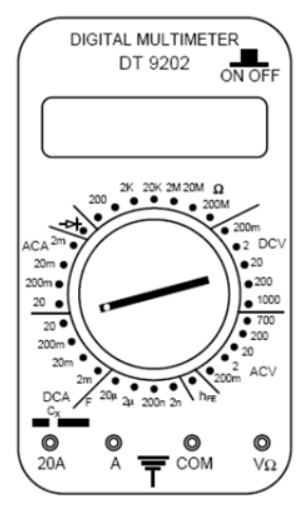
\includegraphics[scale=0.8]{VN12-PH-24-A-014.1 - 1.jpg}
\end{center}

Thứ tự đúng các thao tác là
\begin{mcq} (2)
	\item a, b, d, c, e, g.
	\item c, d, a, b, e, g.
	\item d, a, b, c, e, g.
	\item d, b, a, c, e, g.
\end{mcq}
}	
\loigiai{\textbf{Đáp án: B.}
	
	Các thao tác khi sử dụng đồng hồ đo điện đa năng hiện số là:
	\begin{itemize}
		\item Vặn đầu đánh dấu của núm xoay tới chấm có ghi 200 V, trong vùng ACV.
		\item Cắm hai đầu nối của dây đo vào hai ổn COM và $\text{V}\Omega$.
		\item Nhấn nút ON OFF để bật nguồn cho đồng hồ.
		\item Cho hai đầu của hai dây đo tiếp xúc với hai đầu đoạn mạch cần đo.
		\item Chờ cho các chữ số ổn định, đọc kết quả đo.
		\item Kết thúc thao tác đo, ấn nút ON OFF để tắt nguồn của đồng hồ.
	\end{itemize}
}
\end{enumerate}
\loigiai{\textbf{Đáp án}
\begin{center}
	\begin{tabular}{|m{2.8em}|m{2.8em}|m{2.8em}|m{2.8em}|m{2.8em}|m{2.8em}|m{2.8em}|m{2.8em}|m{2.8em}|m{2.8em}|}
		\hline
		1. B & 2. A & 3. D & 4. D & 5. B & 6. C  & 7. C  & 8. A & 9. C & 10. B\\
		\hline
	\end{tabular}
\end{center}}